\section{Methodology}
\subsection{Dataset Description}
The Dataset at ’Mendeley data’ was designed to be used as a a benchmark for machine learning based phishing detection systems. The dataset includes 11430 URLs with 87 extracted features. The dataset is balanced, it contains exactly 50\% phishing and 50\% legitimate URLs. The Datasets was constructed as of May 2020.\\\\
Link: {\small \url{https://data.mendeley.com/datasets/c2gw7fy2j4/3}}\\
It has features from three different classes:
\begin{itemize}
    \item[-] 56 extracted from the structure and syntax of URLs,
    \item[-] 24 extracted from analyzing their HTML contents,
    \item[-] and 7 were extracted by querying external services.
\end{itemize}
The datasets are divided into 2:
\begin{itemize}
    \item[-] Dataset A: contains a list a URLs together with their
            Document Object Model (DOM) tree objects
    \item[-] Dataset B: contains the extracted feature values that can
            be used directly as input to classifiers for examination.
\end{itemize}
\subsection{Machine Learning Models}
\subsubsection{Support Vector Model}
It is a part of Supervised Learning paradigm.\\
The objective function has two parts: the first aims to maximize the separation between classes, while the second works to minimize misclassifications. The parameter ”C” is the cost assigned to mistakes, treating errors in both positive and negative cases equally.\\
\textit{Objective Function:}
\begin{align}
    \min_{} \left( ||w||^2 + C \sum_{i=1}^n \xi_i \right),\\ 
    \text{where,\quad} y_i (w \cdot f(x_i) + b) \geq 1 - \xi_i \quad 
    \text{and} \quad \xi_i \geq 0
\end{align}
\subsubsection{Logistic Regression}
It is a part of Supervised Learning paradigm.\\
The algorithm applies the logistic function (sigmoid) to a linear combination of input features, producing a probability score. A threshold is then set to classify instances into one of the two classes.\\
\textit{Objective Function:}
\begin{equation}
    J(\theta) = -\frac{1}{m} \sum_{i=1}^m \left[ y^{(i)} \log(h_\theta(x^{(i)})) + (1 - y^{(i)}) \log(1 - h_\theta(x^{(i)})) \right]
\end{equation}
$h_\theta(x^{(i)})$ is the sigmoid (logistic) function applied to the
linear combination of input features x.
\subsubsection{Decision Tree}
It is a part of Supervised Learning paradigm\\.
It works by recursively partitioning the data into subsets based on the most significant attribute at each node. The goal is to create a tree-like structure where each internal node represents a decision based on a feature, each branch represents the outcome of that decision, and each leaf node represents the final prediction or value.\\
\textit{Objective Function:} Decision tree does not have a single objective function that summarizes the entire tree-building process, but you can express the impurity or information gain at a specific node using a criterion such as Gini impurity or entropy.
\begin{align}
    \text{Gini index } G &= \sum_c \Pi_c (1 - \Pi_c)\\
    \text{where } \Pi_c &= \frac{\text{no.of points in the subspace with label c}}{\text{no.of points in the subspace}}
\end{align}
\subsubsection{Random Forest}
It is a part of Supervised Learning paradigm.\\
Random Forest is an ensemble learning method that combines the predictions of multiple decision trees to improve overall performance and robustness. It operates by constructing a multitude of decision trees during training
and outputs the mode (classification) or average (regression) prediction of the individual trees. Random Forests introduce randomness in two key ways: by using a random subset of the training data for each tree (bootstrapping) and by considering a random subset of features at each split. This helps reduce overfitting and increases the model’s generalization ability.\\
\textit{Objective Function:} As it is a ensemble of decision
trees there isn’t a single objective function that summarizes
the entire Random Forest; instead, the focus is on the
individual decision trees and their combination.
\subsection{Performance Metrics}
We use the following metrics to compare the models:
\begin{itemize}
    \item[-] \textbf{Time Taken:} Measures the computational efficiency of each model, indicating the duration required for training and prediction.
    \item[-] \textbf{Accuracy:} Calculates the proportion of correctly classified instances, providing an overall measure of model correctness.
    \item[-] \textbf{Macro F1 Score:} Computes the harmonic mean of precision and recall across all classes, offering a balanced assessment of performance, particularly in imbalanced datasets.
    \item[-] \textbf{Recall:} Measures the model's ability to correctly identify all instances of a given class, indicating its sensitivity.
    \item[-] \textbf{Log Loss:} Evaluates the model's probabilistic predictions, penalizing incorrect classifications with higher confidence.
    \item[-] \textbf{Confusion Matrix:} Visualizes the model's classification performance, showing the counts of true positives, true negatives, false positives, and false negatives for each class.
\end{itemize}
\subsection{Workflow}
\subsubsection{Extracting the data}
We get the ’x’ value by dropping the columns ‘URL’ and ‘status’ from the dataset. ’y’ value from the status column of the dataset by assigning ‘1’ for legitimate and ‘0’ for phishing.
\subsubsection{Splitting the data for Training and  Testing}
The data is split into training and testing/validation data, with 30\% of the data as testing data. This is done using the \textit{'train\_test\_split'} function available in the \textit{sklearn.model\_selection} library.
\subsubsection{Raw Data vs Scaled Data}
\textit{Data Scaling:} Standardization is used to scale the ’X’ values, centering it around a mean with a unit standard deviation. We use the ’fit trasfrom’ and ’transform’ function within ’StandardScalar’ class to standardize the training data and test data respectively.\\
This analysis aims to evaluate the impact of data scaling on model performance relative to the use of raw data.
\subsubsection{Cross Validation}
\textit{K-fold cross-validation} assesses a model's generalization by partitioning the data into 'k' subsets (folds). It iteratively trains and tests the model 'k' times, using each fold once as the test set and the rest as training data. The averaged performance across all iterations provides a more reliable estimate of generalization, effectively reducing overfitting, bias, and variance compared to a single train-test split. We employ 10-fold cross-validation.\\
\textit{Average Accuracy:} Provides a more robust evaluation of model performance than standard accuracy, mitigating overfitting due to the train-test split.\\
\textit{Variance:} Quantifies model sensitivity to training data variations, indicating the extent of overfitting introduced by the train-test split.
\subsubsection{Hyperparameter Tuning}
\begin{tabular}{ll}
\textbf{Support Vector Model:} & \textbf{Logistic Regression:} \\
\ kernel: ['linear', 'rbf'] & \ penalty: ['l1', 'l2'] \\
\ C: [1, 10, 20] & \ C: np.logspace(0, 10, 6) \\
\ gamma: ['auto', 'scale'] & \\
& \\
\textbf{Decision Tree:} & \textbf{Random Forest:} \\
\ max\_depth: [25, 30, 25] & \ max\_depth: [20, 25, 30] \\
\ min\_samples\_leaf: [1, 5, 10] & \ max\_leaf\_nodes: [400, 450, 475] \\
\ min\_samples\_split: [25, 30, 35] & \ min\_samples\_split: [1, 5] \\
\end{tabular}\\\\\\
\textit{GridSearchCV} is a technique in machine learning that systematically explores a predefined hyperparameter grid to find the optimal configuration for a model. It uses 'k-fold cross-validation', we use k = 10, to evaluate the performance of each combination of hyperparameters and selects the best parameters based on average performance.
\subsubsection{Majority Voting}
\textit{Majority voting}, implemented using scikit-learn's "VotingClassifier", combines predictions from our four models. Hard voting selects the most frequently predicted class, while soft voting averages predicted probabilities, choosing the class with the highest average. In particular, soft voting allows for the application of weights to individual models, reflecting their relative confidence or performance.
\begin{figure}[ht!]
    \centering
    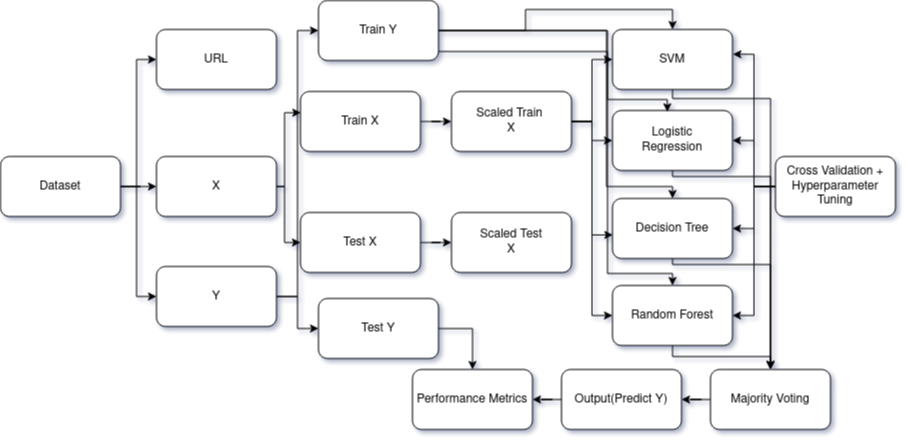
\includegraphics[width = 0.45\textwidth]{./images/workflow.png}
    \caption{Workflow}
    \label{fig:2}
\end{figure}